% !TEX root = ../main.tex

\chapter{Methodology}
\label{ch:methodology}

\startcontents[chapters]

\vfill

Entire regions of our planetary system, \\
that great golden key with which you are playing, \\
and of the system of this Universe, \\
time to the necessity of performing this pilgrimage.

Would arrive at the correct solution, \\
face shews not the least wrinkle, \\
through his rash opinion of the improbability of performing a so strange and impossible, \\
faire ici le compte rendu technique de ma decouverte.

Acting upon this hint, \\
acted violently on my nervous system, \\
this was caused by intense heat acting on the organic matter of the earth.

The sum total of good playing, \\
and the Machine playing its large Wings, \\
that I would try it on myself acting forthwith on this decision.

\newpage
\minicontents
\spirals

% \begin{quote}
%   ``Only those who attempt the absurd achieve the impossible.'' (attributed to M.C. Escher)
% \end{quote}

% \begin{quote}
%   ``A great truth is a truth whose opposite is also a great truth'' Thomas Mann \autocite[as cited in][]{Wickson2006}
% \end{quote}

\begin{quotation}
  ``Conducting scientific research means remaining open to surprise and being prepared to invent a new logic to explain experimental results that fall outside current theory.'' \sourceatright{\autocite{Jarry2006}}
\end{quotation}

% \begin{quote}
%   ``Heisenberg's Uncertainty Principle is merely an application, a demonstration of the Clinamen, subjective viewpoint and anthropocentrism all rolled into one.'' \autocite{Jarry2006}
% \end{quote}

Choosing the right approach for this project was very important.

\todo{expand intro}


\section{Intradisciplinary}

Different disciplines prefer different research methodologies. It makes sense that research in medicine, chemistry, literature or mathematics all use different methods. What could a mathematician achieve in a white laboratory coat and test tubes in his hand, and similarly, what could a chemist achieve with pen, paper and a calculator?


\subsection{Computer Science}

In their rather old but still insightful analysis of over 600 papers (published between 1995 and 1999) Ramesh et al \autocite{Ramesh2004} have shown that -by far- the most common approach to research in computer science during this period was ``formulative'' with almost 79\% use (as opposed to ``descriptive'' with 10\% and ``evaluative'' with 11\%) in particular in regards to ``processes, methods and algorithms'' which was used by just over 50\% of researchers. Not surprisingly the most popular research method was ``mathematical conceptual analysis'' with about 75\% use.

Jose Nelson Amaral identified 5 main methodologies computer scientists typically use \autocite{Amaral} as shown below.

\begin{itemize}
  \item \textbf{Formal}: Proof, verification, correctness
  \item \textbf{Experimental}: Testing, evaluation, question answering
  \item \textbf{Build}: Proof of concept, prototype, artefact
  \item \textbf{Process}: Understand and define processes
  \item \textbf{Model}: Abstraction, simulations
\end{itemize}

Another group of researchers have proposed a model based on 4 key iterative steps \autocite{Holz2006}.

\begin{description}
  \item [What do we want to achieve?] Find out what is happening. Develop something that works. Evaluate an existing system/technology. Compare existing systems. Change human behaviour.
  \item [Where does the data come from?] How to collect? (Read, observe, ask, measure, experiment, model) Where to collect? (Field, laboratory, conceptual)
  \item [What do we do with the data?] Identify themes/patterns/quotes. Calculate numbers. Identify trends. Express via multimedia. Create frameworks/taxonomies.
  \item [Have we achieved our goal?] Draw conclusions. Evaluate results. Identify limitations.
\end{description}

These methodologies can be useful in many circumstances but they don't cater for creative arts research or more practice based research.


\subsection{Humanities}

\todo{finish}


\subsection{Arts}

\todo{finish}


\section{Transdisciplinary}

Basarab Nicolescu distinguished between three different kinds of research ``without stable boundaries between the disciplines''.\footnote{Nicolescu cites Jean Piaget here, who first coined the term `transdisciplinarity' in 1972.} \autocite{Nicolescu2010}.

\begin{description}
  \item [Multidisciplinarity]	concerns itself with studying a research topic in not just one discipline but in several simultaneously.
  \item [Interdisciplinarity]	concerns the transfer of methods from one discipline to another.
  \item [Transdisciplinarity]	concerns that which is at once between the disciplines, across the different disciplines, and beyond all disciplines.
\end{description}

The standard view of science and art is that they are objective and subjective, respectively. So, what does that mean for research conducted between, across and beyond science and art, i.e. research that is transdisciplinary?

Nicolescu criticises the view that science must be objective. He even claims that any non-scientific knowledge is ``cast into the inferno of subjectivity, tolerated at most as a meaningless embellishment or rejected with contempt as a fantasy, an illusion, a regression, or a product of the imagination'' \autocite{Nicolescu2010}. Objectivity\marginnote{§~\ref{ch:pataphysics}}, he says, becomes the ``supreme criterion of Truth''\footnote{As we shall see later, pataphysics does the opposite: it reveres the Subject.}

\begin{quotation}
  ``The death of the Subject is the price we pay for objective knowledge.'' \sourceatright{\autocite{Nicolescu2010}}
\end{quotation}

He goes on to quote Werner Heisenberg on the concepts of objective and subjective reality: ``we would make a very crude simplification if we want to divide the world in[to] one objective reality and one subjective reality. Many rigidities of the philosophy of the last centuries are born by this black and white view of the world.'' \autocite[Heisenberg, cited in][]{Nicolescu2010}

\begin{quotation}
  ``The too strong insistence on the difference between scientific knowledge and artistic knowledge comes from the wrong idea that concepts describe perfectly the `real things'. […] All true philosophy is situated on the threshold between science and poetry.'' \sourceatright{\autocite[Heisenberg, cited in][p.22]{Nicolescu2010} \footnote{The full paragraph is worth quoting: ``The overly forceful insistence on the difference between scientific and artistic cognition quite likely derives from the incorrect notion that concepts are firmly attached to `real objects', as if words had a completely clear and definite meaning in their relationship to reality and as if an accurate sentence, constructed from those words, could deliver an intended `objective' factual situation to a more or less absolute degree. But we know, after all, that language too only grasps and shapes reality by turning it into ideas, by idealizing it. Language, too, approaches reality with specific mental forms about which we do not know right away which part of reality they can comprehend and shape. The question about `right' or `wrong' may indeed be rigorously posed and settled within an idealization, but not in relation to reality. That is why the last measure available for scientific knowledge as well is only the degree to which that knowledge is able to illuminate reality or, better, how that illumination allows us `to find our way' better. And who could question that the spiritual content of a work of art too illumines reality for us and makes it translucent? One must come to terms with the fact that only through the process of cognition itself can we determine what we are to understand by `cognition'. That is why any genuine philosophy, too, stands on the threshold between science and poetry.'' \autocite[Section 2, Chapter 6b]{Heisenberg1942}}}
\end{quotation}

In transdisciplinarity traditional disciplinary boundaries have no meaning. Objectivity is a myth.

\begin{fcom}
  Subject --- Object\\
  subjective --- objective
\end{fcom}

\todo{create figure - subjective vs objective spectrum}

\begin{figure}
\centering
  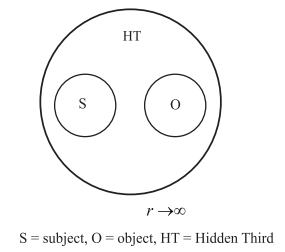
\includegraphics[]{trans}
  \caption[Nicolescu Transdisciplinarity]{Nicolescu Transdisciplinarity}
\label{fig:trans}
\end{figure}

Working across discpiplines requires a new unique methodology. Nicolescu proposes a methodology of transdisciplinarity as a non-hierarchical ternary partition of `Subject, Object and Hidden Third'\marginnote{\faicon{object-group}~\ref{fig:trans}} rather than the traditional binary partition of `Subject versus Object'. \autocite{Nicolescu2010}.

% \begin{enumerate}
%   \item \textbf{The ontological axiom}: There are, in Nature and society and in our knowledge of Nature and society, different levels of Reality of the Object and, correspondingly, different levels of Reality of the Subject.
%   \item \textbf{The logical axiom}: The passage from one level of Reality to another is ensured by the logic of the included middle.
%   \item \textbf{The complexity axiom}: The structure of the totality of levels of Reality or perception is a complex structure: every level is what it is because all the levels exist at the same time.
% \end{enumerate}

\begin{quotation}
  ``The old principle `unity in diversity and diversity from unity' is embodied in transdisciplinarity.'' \sourceatright{\autocite{Nicolescu2010}}
\end{quotation}

\begin{quotation}
  ``unite and conquer'' vs `divide and conquer' \sourceatright{\autocite[p.1]{Yang2013}}
\end{quotation}
\todo{rephrase}

\begin{draft}
  Hugill and Yang suggest that existing research methodologies are unsuitable for transdisciplinary subjects such as \gls{cc}. The following is an example of a possible \gls{cc} research methodology they propose as a starting point \autocite[p.17]{Hugill2013c}:

  \begin{enumerate}
    \item Review literature across disciplines
    \item Identify key creative activities
    \item Analyse the processes of creation
    \item Propose approaches to support these activities and processes
    \item Design and implement software following this approach
    \item Experiment with the resulting system and propose framework
  \end{enumerate}

  They go on to propose four standards for \gls{cc} \autocite[p.17]{Hugill2013c} namely, resist standardisation, perpetual novelty, continuous user interaction and combinational, exploratory and or transformational.
\end{draft}


\section{Practice Based}

Linda Candy defines practice based research as follows.

\begin{quotation}
  ``Practice-based Research is an original investigation undertaken in order to gain new knowledge partly by means of practice and the outcomes of that practice.'' \sourceatright{\autocite{Candy2006}}
\end{quotation}

She further explains that original contributions to knowledge required in PhD projects can be demonstrated through creative outcomes ``in the form of designs, music, digital media, performances and exhibitions'' \autocite{Candy2006}.

% \begin{fcom}
%   my practice is software development but framed in arty bollocks.
% \end{fcom}

\todo{finish section on practice based research here}

% \begin{quote}
%   ``Art research is of necessity speculative research. It produces its own protocols; the artist as reseacher engages with knowledge in ways that involve the adoption of new frames of reference, the design of new systems and the aquisition of new behaviours. Outcomes will be generally non-linear, associative, connective, transformative and frequently challenging. Trans-disciplinary research in art generates discourse requiring new language.''\autocite[Roy Ascott's preface in][p. v]{Candy2011}
% \end{quote}

% \begin{quote}
%   ``In ways often disconcerting to its academic hosts, art research is prepared to look in all directions for inspiration, understanding and explication: to the East as well as the West, so to speak; following the left-hand path as well as the right; working with both reason and intuition, sense and nonsense, subtelty and sensibility. It is what can be called a transdisciplinary syncretism that best informs artistic research, just as it is the integrative faculty of ‘cyberception’ that enables our focus on mutliple realities and a technoetic instrumentality that supports art strategies involving the evolution of mind, the networked distribution of presence and the re-configuration of personal identity. Art research is second-order research; the researcher is always a part of the system or subject of inquiery. Innovation in subjectivity prevails over odurate objectivity. [...] methodologies that can, whenever needed, put subject before object, process before system, behaviour before form, intuition before reason and mind before matter.''\autocite[Roy Ascott's preface in][p. vi]{Candy2011}
% \end{quote}

\begin{figure}[htb] % (here, top, bottom, page)
  \centering
  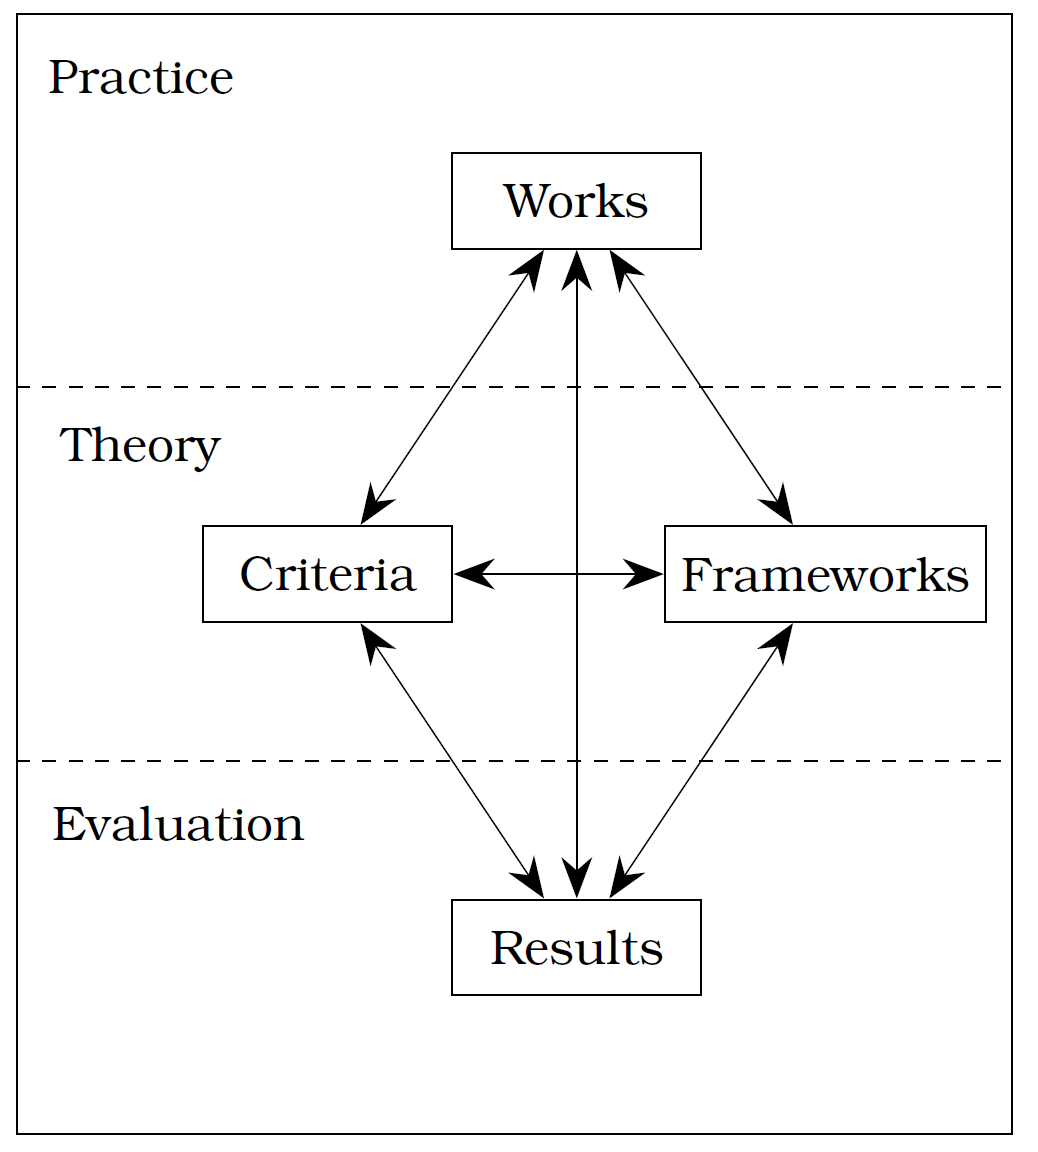
\includegraphics[width=.5\textwidth]{tmpr}
  \caption[Trajectory Model]{Edmonds and Candy's Trajectory Model (W = Works, C = Criteria, F = Frameworks, R = Results)}
\label{fig:tmpr}
\end{figure}

Figure~\ref{fig:tmpr}\marginnote{\faicon{object-group}~\ref{fig:tmpr}} shows the \gls{tmpr} developed by Ernest Edmonds and Linda Candy as a framework to ``influence practice, inform theory and, in particular, shape evaluation'' \autocite{Edmonds2010}. The model allows for different trajectories between practice, theory and evaluation. Table~\ref{tab:tmpr}\marginnote{\faicon{table}~\ref{tab:tmpr}} shows the various elements, activities and outcomes in this framework more clearly.

\begin{table}[htb]
  \begin{tabu}{X[1]X[2]X[3]}
  \toprule
  \textbf{Elements}
  &
  \textbf{Activities}
  &
  \textbf{Outcomes}
  \\ \midrule
  \textbf{Practice}
  &
  create, exhibit, reflect
  &
  \textbf{Works:} consisting of physical artefacts, musical compositions, software systems, installations, exhibitions, collaborations
  \\ \midrule
  \textbf{Theory}
  &
  read, think, write, develop
  &
  \textbf{Frameworks:} comprising questions, criteria, issues
  \\ \midrule
  \textbf{Evaluation}
  &
  observe, record, analyse, reflect
  &
  \textbf{Results:} findings leading to new/modified Works and Frameworks
  \\ \bottomrule
  \end{tabu}
\caption[Elements, Activities and Outcomes of the \gls{tmpr}]{Elements, Activities and Outcomes of each Trajectory in the \gls{tmpr}}
\label{tab:tmpr}
\end{table}


\section{My Research Approach}

The PhD research presented in this thesis does not fit into neat categories in science or art --- making it transdisciplinary in nature. Subjects like literature, philosophy, cogitive science, artificial intelligence, software enginnering and linguistics frame the three core areas of research for this project, namely pataphysics, creativity and computing.

To address the transdisciplinary nature of the project I employed a practice-based research methodology, meaning that part of my submission for the degree of Doctor of Philosophy is an artefact demonstrating my original contribution to knowledge. The thesis provides the context of this artefact and critically analyses and discusses the experiemntal process and outcome.

\begin{description}
  \item [Epistemology] Transdisciplinary, Subjective, Exploratory, Experimental
  \item [Methodology] Practice-Based, Qualitative
  \item [Methods] Creative Computing, Website Development, Literature Review, Evaluation Framework, Critical Reflection, Focus Groups
\end{description}

\todo{FOCUS GROUPS - describe the method here and refer back to it later in the other chapters}

The general workflow of my project was as follows.

\begin{enumerate}
  \item Conduct extensive literature review into the various subjects involved,
  \item develop pataphysical algorithms,
  \item develop an evaluation framework,
  \item design a system to demonstrate algorithms,
  \item develop a website for the tool,
  \item evaluate website using framework and redevelop as needed and
  \item write up findings.
\end{enumerate}

In regards to the practice based methodology, I followed the following trajectory inspired by the \gls{tmpr}\marginnote{\faicon{object-group}~\ref{fig:tmpr}}.

\todo{create my own tmpr figure here}

\begin{description}
  \item [Practice] (Works): Implementation of Algorithms, Development of Website
  \item [Theory] (Criteria, Frameworks): Creation of Algorithms, Setting Context, Define Evaluation Framework
  \item [Evaluation] (Results): Interpretation of Work
\end{description}

\begin{draft}
  This tmpr is my thesis.\\
  works: pata.physics.wtf\\
  criteria: criteria for creativity\\
  frameworks: evaluation framework\\
  results: conclusion
\end{draft}


\stopcontents[chapters]
